\documentclass[11pt]{article}
\usepackage{geometry}
\geometry{a4paper}
\usepackage{graphicx}
\usepackage{epstopdf}
\usepackage[slovene]{babel}
\usepackage[utf8]{inputenc}
\usepackage{natbib}
\usepackage{float}
\DeclareGraphicsRule{.tif}{png}{.png}{`convert #1 `dirname #1`/`basename #1 .tif`.png}


\title{Seminarska naloga \\ Zmogljivost računalniških sistemov}
\author{Gregor Vitek, Žan Palčič, Maj Smerkol\\
\
\\Zanesljivost in zmogljivost računalniških sistemov\\
Fakulteta za računalništvo in informatiko, Univerza v Ljubljani}
\date{\today}                                          

\begin{document}
\maketitle

\paragraph*{Ključne besede:}
Zmogljivost, benchmark, storitve v oblaku, strežniki

\section{Uvod}

\begin{figure}[H]
\centerline{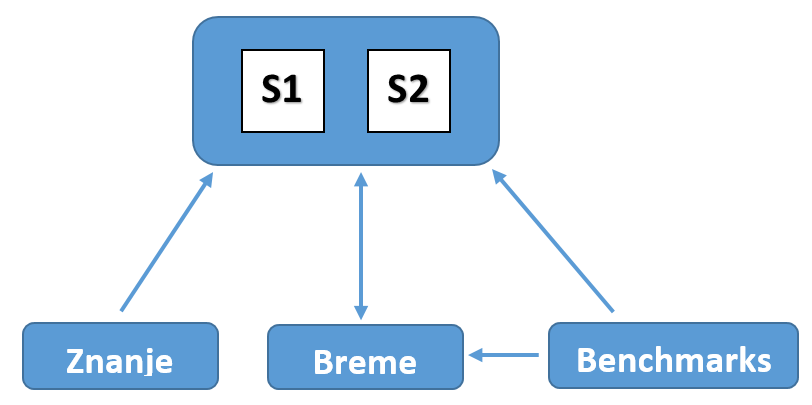
\includegraphics[scale=0.5]
{vzorec.PNG}}
\caption{Odvisnost izbire S1 in S2 glede na podane atribute.}
\label{fig:miselni}
\end{figure}
\subsection{Benchmarks}

Na spletu lahko najdemo že opravljene znane benchmarke\cite{Benchmarks}, ki ocenjujejo določene lastnosti oblačnih sistemov (S2). Tu lahko najdemo podatke o procesni moči sistema, ki ga dobimo v uporabo, količini pomnilnika na takšnem sistemu in zmogljivosti opravljanja nekaterih znanih testov, kot so naprimer urejanje velike količine podatkov. Te meritve, ki jih lahko preberemo med že opravljenimi testi, pa ne kažejo na zmogljivost neke določene storitve, kot jo doživlja uporabnik, ampak samo povejo, kako zmogljiva je strojna oprema, ki jo dobimo na voljo. Končnega uporabnika storive pa ponavadi zanima predvsem hitrost odzivanja, ki je odvisna od več parametrov.
Med slednje spadajo hitrost in latenca povezave od naprave uporabanika (end point) do fizične lokacije oblačne storitve ali strežnika, velikost poslanega zahtevka, hitrost odbelave zahtevka, hitrost in latenca poslanega odgovora iz oblaka ali strežnika proti uporabniku in drugo. Pri tem lahko lahko nekatere storitve implementiramo na tak način, da uporabnik verjame, da je odzivni čas veliko manjši, kot dejansko je (naprimer shranjevanje datotek na disk v oblaku). Na končno uporabnikovo izkušnjo hitrosti pa vpliva tudi zmogljivost naprave, ki predstavlja njegovo dostopno točko. 

Kot omenjeno zgoraj se na spletu najdejo seznami spletnih sistemov, ki jih lahko uporabniki med seboj primerjajo. Primerjajo lahko rezultate za različne parametre kot so hitrost procesorja pri računanju s plavajočo vejico ali celimi števili, hitrost prenosa pri branju podatkov oz. pisanju na pomnilnih enotah, hitrost prenosa podatkov lokalno znotraj oblačne storitve in drugo. Pri testiranju teh parametrov se lahko uporabi različna orodja kot so SPEC CPU 2006, Test Harness, TeraSort, Geekbench in še mnogo drugih. Pri sami izbiri programov se moramo osredotočiti tudi na bremena, ki jih lahko s posameznim programom definiramo in tako testiramo željene parametre. Ključen kriterij poleg kakovosti storitev in definiranje bremen je tudi cena. Zaželjeni so prosto dostopni oz. zastonjski progami. 

Pri testiranju spletnih strežnikov (S1) uporabnika navadno  zanima število zahtev, ki jih strežnik obdela, latenca oz. čas odziva strežnika za novo povezavo ali zahtevek, in količina prenesenih podatkov v sekundi, glede na različne parametre (velikost, shranjevanje v predpomnilnik, različna pasovna širina). Za izvajanje stresnih testov se na spletu nahaja veliko orodij, ki lahko pridejo v pomoč (Apachech, Apache JMeter, Curl-loader, OpenSTA …). 

\subsection{Znanje}
Člani te skupine imamo predznanje iz arhitekture in organizacije računalniških sistemov, kot so procesne enote, pomnilniška hierarhija in vhodno/izhodne naprave. Poznamo tudi paralelno programiranje na različnih platformah v jeziku C, kar bi nam lahko pomagalo pri optimizaciji določenih storitev. Imamo predznanje iz strežniških arhitektur in osnov spletne komunikacije. Imamo tudi omejene izkušnje uporabe PaaS (platform as a service) za postavitev spletnih strani in postavitve podakovnih baz na teh strežnikih. Nimamo pa izkušenj s testiranjem in merjenjem zmogljivosti katerega koli on naštetih modelov.

\subsection{Izbira ciljnih sistemov}
Za ciljni sistem bi izbrali kakšnega od večjih ponudnikov oblačnih storitev kot so Google Cloud, Amazon web service, Microsoft Azure, lahko tudi kakšne manjše kot so Rackspace. Večina teh ponudnikov ima omejene zastonjska testna obdobja, med katerimi bi lahko izvedli meritve.
Ker imamo dostop do računalnika Raspberry Pi \footnote{http://www.raspberrypi.org/} in predvsem zastonjskih verzij oblačnih storitev, nas zanima primerjava med temi platformami. Raspberry Pi je računalnik, ki stane okrog 30 evrov in ne porabi praktično nič elektrike, v zameno pa ponuja primerno majhno zmogljivost. Ne plačljive oblačne storitve pa so močno časovno omejene ali pa ponujajo prav tako zelo majhne zmogljivosti.
Zaradi naših predznanj bi lahko storitev za strežnik, katerega ustroj in delovanje poznamo, najbrž bolje optimizirali, kot oblačno storitev, kar je prev tako vredno preveriti.

\subsection{Breme in cilj primerjave}
Če se bomo odločili za primerjanje zmogljivosti in cene med oblačnimi storitvami in strežnikom na platformi Raspberry Pi bomo predvsem iskali najcenejšo rešitev. Ker pa se za različne storitve in aplikacije zahteve po zmogljivosti strojne opreme lahko dramatično razlikujejo, bi bilo dobro primerjati na teh dveh platformah več čimbolj različnih storitev. 

Po izbiri teh storitev bomo tudi lahko izbrali primerna bremena za testiranje teh storitev. Za primerjati različne aspekte izbranih sistemov, bi bilo dobro testirati eno račlunsko zahtevno storitev, eno storitev, ki bi bolj obremenila delovni pomnilnik, na primer urejanje podatkov ali kaj podobnega, in eno storitev, ki bi bolj kot sistem obremenila omrežje, naprimer prenos večje količine podatkov. S tem tretjim testom bi izvedeli, koliko na delovanje sistemov vpliva omrežje, ki ga ne moremo spremeniti, ko želimo ustvariti neko storitev, lahko pa morda vpliva na maksimalno dosegljivo kvaliteto storitve, kot jo vidi končni uporabnik.

\newpage
\section{Sistem}
\begin{figure}[H]
\centerline{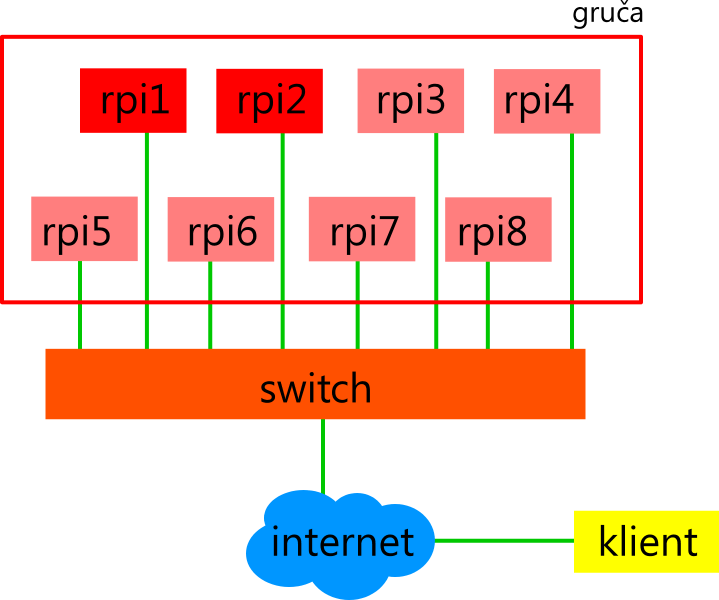
\includegraphics[scale=1.5]
{shemaSistema.png}}
\caption{Shema sistema. Rdeči kvadrati so računalniki Raspberry Pi, bledo rdeči še niso dodani.}
\label{fig:gruca}
\end{figure}

Naš sistem je gruča računalnikov, narejena po vzoru Beowulf gruč. Namenjena je zaganjanju porazdeljenih programov. Trenutno sta v mrežo povezana dva računalnika Raspberry Pi, model 1B in model 1B+. V gruči je trenutno samo en. Do njega imamo SSH dostop tudi z zunanjega omrežja.
Do tega sistema bomo dostopali s klientov, ki bodo izven lokalnega omrežja. Gručo bomo uporabljali kot računski strežnik, ki bo po zahtevi klienta izvajal porazdeljeno hitro Fourierjevo transformacijo. Klient po prek omrežja poslal podatke v obliki glasbene datoteke, gruča bo podatke prejela (oziroma jih bo master računalnik v gruči) in izvajanje algoritma porazdelil prek vseh računalnikov v gruči, vključno s sabo.
Testirali smo dostop do gruče od zunaj in delovanje sistema MPI na računalniku rpi1. To smo storili tako, da smo na njem poganjali z MPI implementiran algoritem porazdeljeni Quicksort (porazdeljeno hitro urejanje\footnote{http://en.wikipedia.org/wiki/Quicksort\#Parallelization}).

Pri povezovanju Raspberry Pi-jev v gručo smo uporabili Message Passing Interface(MPI), ki je standard za izmenjevanje sporočil med računalniki oz. procesih v več-računalniških sistemih, gručah in delovnih postajah. Omogoča komunikacijo točka-točka, skupinske komunikacije, spremljanje delovanja in tudi spreminjanje topologije za posamezen program. MPI je standard, ki omogoča velik nabor funkcij, vendar za uporabo standarda ni potrebno poznati vseh. Pri sami komunikaciji računalniki med seboj uporabljajo implementacijo MPICH2 \cite{Mpich},
ki je zelo razširjena programska knjižnica poleg tega pa je enostavna za vzpostavitev in uporabo. Na vsakem računalniku je implementacija 
MPICH2 in datoteka (machinefile)\cite{Gruca} v kateri so zapisani IP naslovien sodelojočih(sosednjih) lokalnih računalnikov, na katere se delo porazdeli.

Začeli smo tudi delo na implementaciji porazdeljenega algoritma FFT, ki ga bomo izvajali na gruči. Alogoritem že deluje, treba pa je še pripraviti paralelizem in branje s socketa (za pridobivanje podatkov z omrežja).

\subsection{Implementacija storitve}
V gručo smo dodali še en Raspberry Pi, tako da zdaj je prava gruča, ne le en računalnik, ki poganja MPI. Raspberry Pi smo pripravili na delovanje v gruči tako, da smo klonirali sliko datotečnega sistema. Potrebni so bili popravki v konfiguraciji omrežja, zdaj deluje pravilno.

Implementirali smo storitev, ki zvočno datoteko pretvori v binarno s pomočjo knjižnjice \texttt{libsndfile}\cite{Audio}. Programa še nismo testirali na gruči, deluje pa na enem računalniku. Testiranje smo izvedli z zvočno datoteko, veliko približno 8 miljonov vzorcev. Program na enem jedru teče zelo počasi, zato upamo, da bo porazdeljeni sistem bolj učinkovit. Vsekakor se ni izpolnil strah, da bi algoritem tekel prehitro, da bi se izplačalo ga poganjati na gruči. Imeli smo nekaj težav s kodiranjem datoteke nazaj v zvočno datoteko.

Pretvorbo izvjamo z rekurzivnim algoritmom FFT. Implementacija je zaradi uporabe razreda ValArray iz knjižnjice STL počasna, če je prevanjanje izvedeno z Microsoft Visual Studio prevajalnikom, vendar bi se moral prevajalnik gcc obnašati bolje. 

\vspace{10pt}

Implementirali smo strežnik, ki sprejema zahtevke z eno ali več datotekami. Strežnik tudi odgovarja, vendar imamo trenutno občasno ne uspe poslati podatkov. Težava ni kritična, nameravamo pa jo odpraviti čim prej. Implementirali smo tudi klienta, ki pošilja zahtevek z eno ali več datotekami.

Program, ki izvaja manipulacije frekvenčnega spektra, smo izboljšali, zdaj upošteva lastnosti Fourierjeve transformacije in deluje pravilno. Zavržemo del frekvenčnega spektra, ki je zrcalna slika relevantnega dela, transformacije, ki jih izvajamo na preostanku so zato bolj smiselne in se obnašajo kot pričakovano.

\vspace{10pt}

% povezovanje v enoten sistem

\section{Meritve}

Naš problem predstavlja veliko računsko breme gruči ampak relativno majhno breme za prenos podatkov prek omrežja. Na enem vozlišču traja obdelovanje 5 sekund zvoka okrog 40 sekund. Algoritem je hitrostnega razreda $O(n log n)$.

Zaradi tipa problema in bremena nas zanimajo časi računanja (procesuranja na gruči, wall-clock time, v odvisnosti od števila uporabljenih vozlišč in velikosti bremena), prenosa podatkov na in iz gruče (latenca omrežja - čas prenosa je najbrž zanemarljiv, saj so datoteke velike med 1MB in 10MB), latence prenosa podatkov med vozlišči v gruči (da vidimo, ali je paralelizacija na gruči primerna ali bi bilo bolje uporabljati paralelizacijo na več jedrih ali podobni arhitekturi) in največje število datotek, ki jih lahko obdeluje hkrati, preden se gruča ali deli nje sesujejo.

Izmerjeni časi: 
\begin{itemize}
\item Procesiranje, 1 vozlišče, n = 5s: približno 40 sekund
\item Procesiranje, 2 vozlišči, n = 5s: približno 20 sekund
\item Procesiranje, 3 vozlišča, n = 5s: približno 19 sekund
\end{itemize}
Razlika med 2 in 3 vozlišči je premajhna, da bi lahko sklepali na pohitritev. Zaradi tipa algoritma (FFT se rekurzivno deli vedno na dva dela, zato deluje dobro le, če uporabljamo $2^n$ paralelnih niti.

\section{Načrt za naprej}

Algoritem bomo poskusili optimizirati, saj smo ugotovili, da deluje zelo počasi in da lahko problem razbijemo na več manjših problemov, ki bi se morali izvajati hitreje, saj za dovolj velik $n$ velja $nlog(n) > nlog(n/m)*m$.
Začeli bomo tudi izvajati eksperimente z različno velikimi bremeni in v različnih okoliščinah. Za rezultat meritev bomo upoštevali najmanjšo, največjo in povprečno meritev.

\bibliographystyle{plain}
\bibliography{literatura}

\newpage
\end{document}